\subsection{1.4. Xây dựng biểu đồ mô tả nghiệp vụ và phân cấp chức năng}

\subsubsection{1.4.1. Biểu đồ hoạt động mô tả luồng nghiệp vụ}
Để mô tả trực quan quy trình phối hợp liên vai trò trong vòng đời tài liệu, luồng hoạt động nghiệp vụ được phân tách qua 4 làn như Hình 1.3:

\begin{figure}[H]
\centering
\IfFileExists{chuong1/images/activity_swimlane_5share.png}{%
    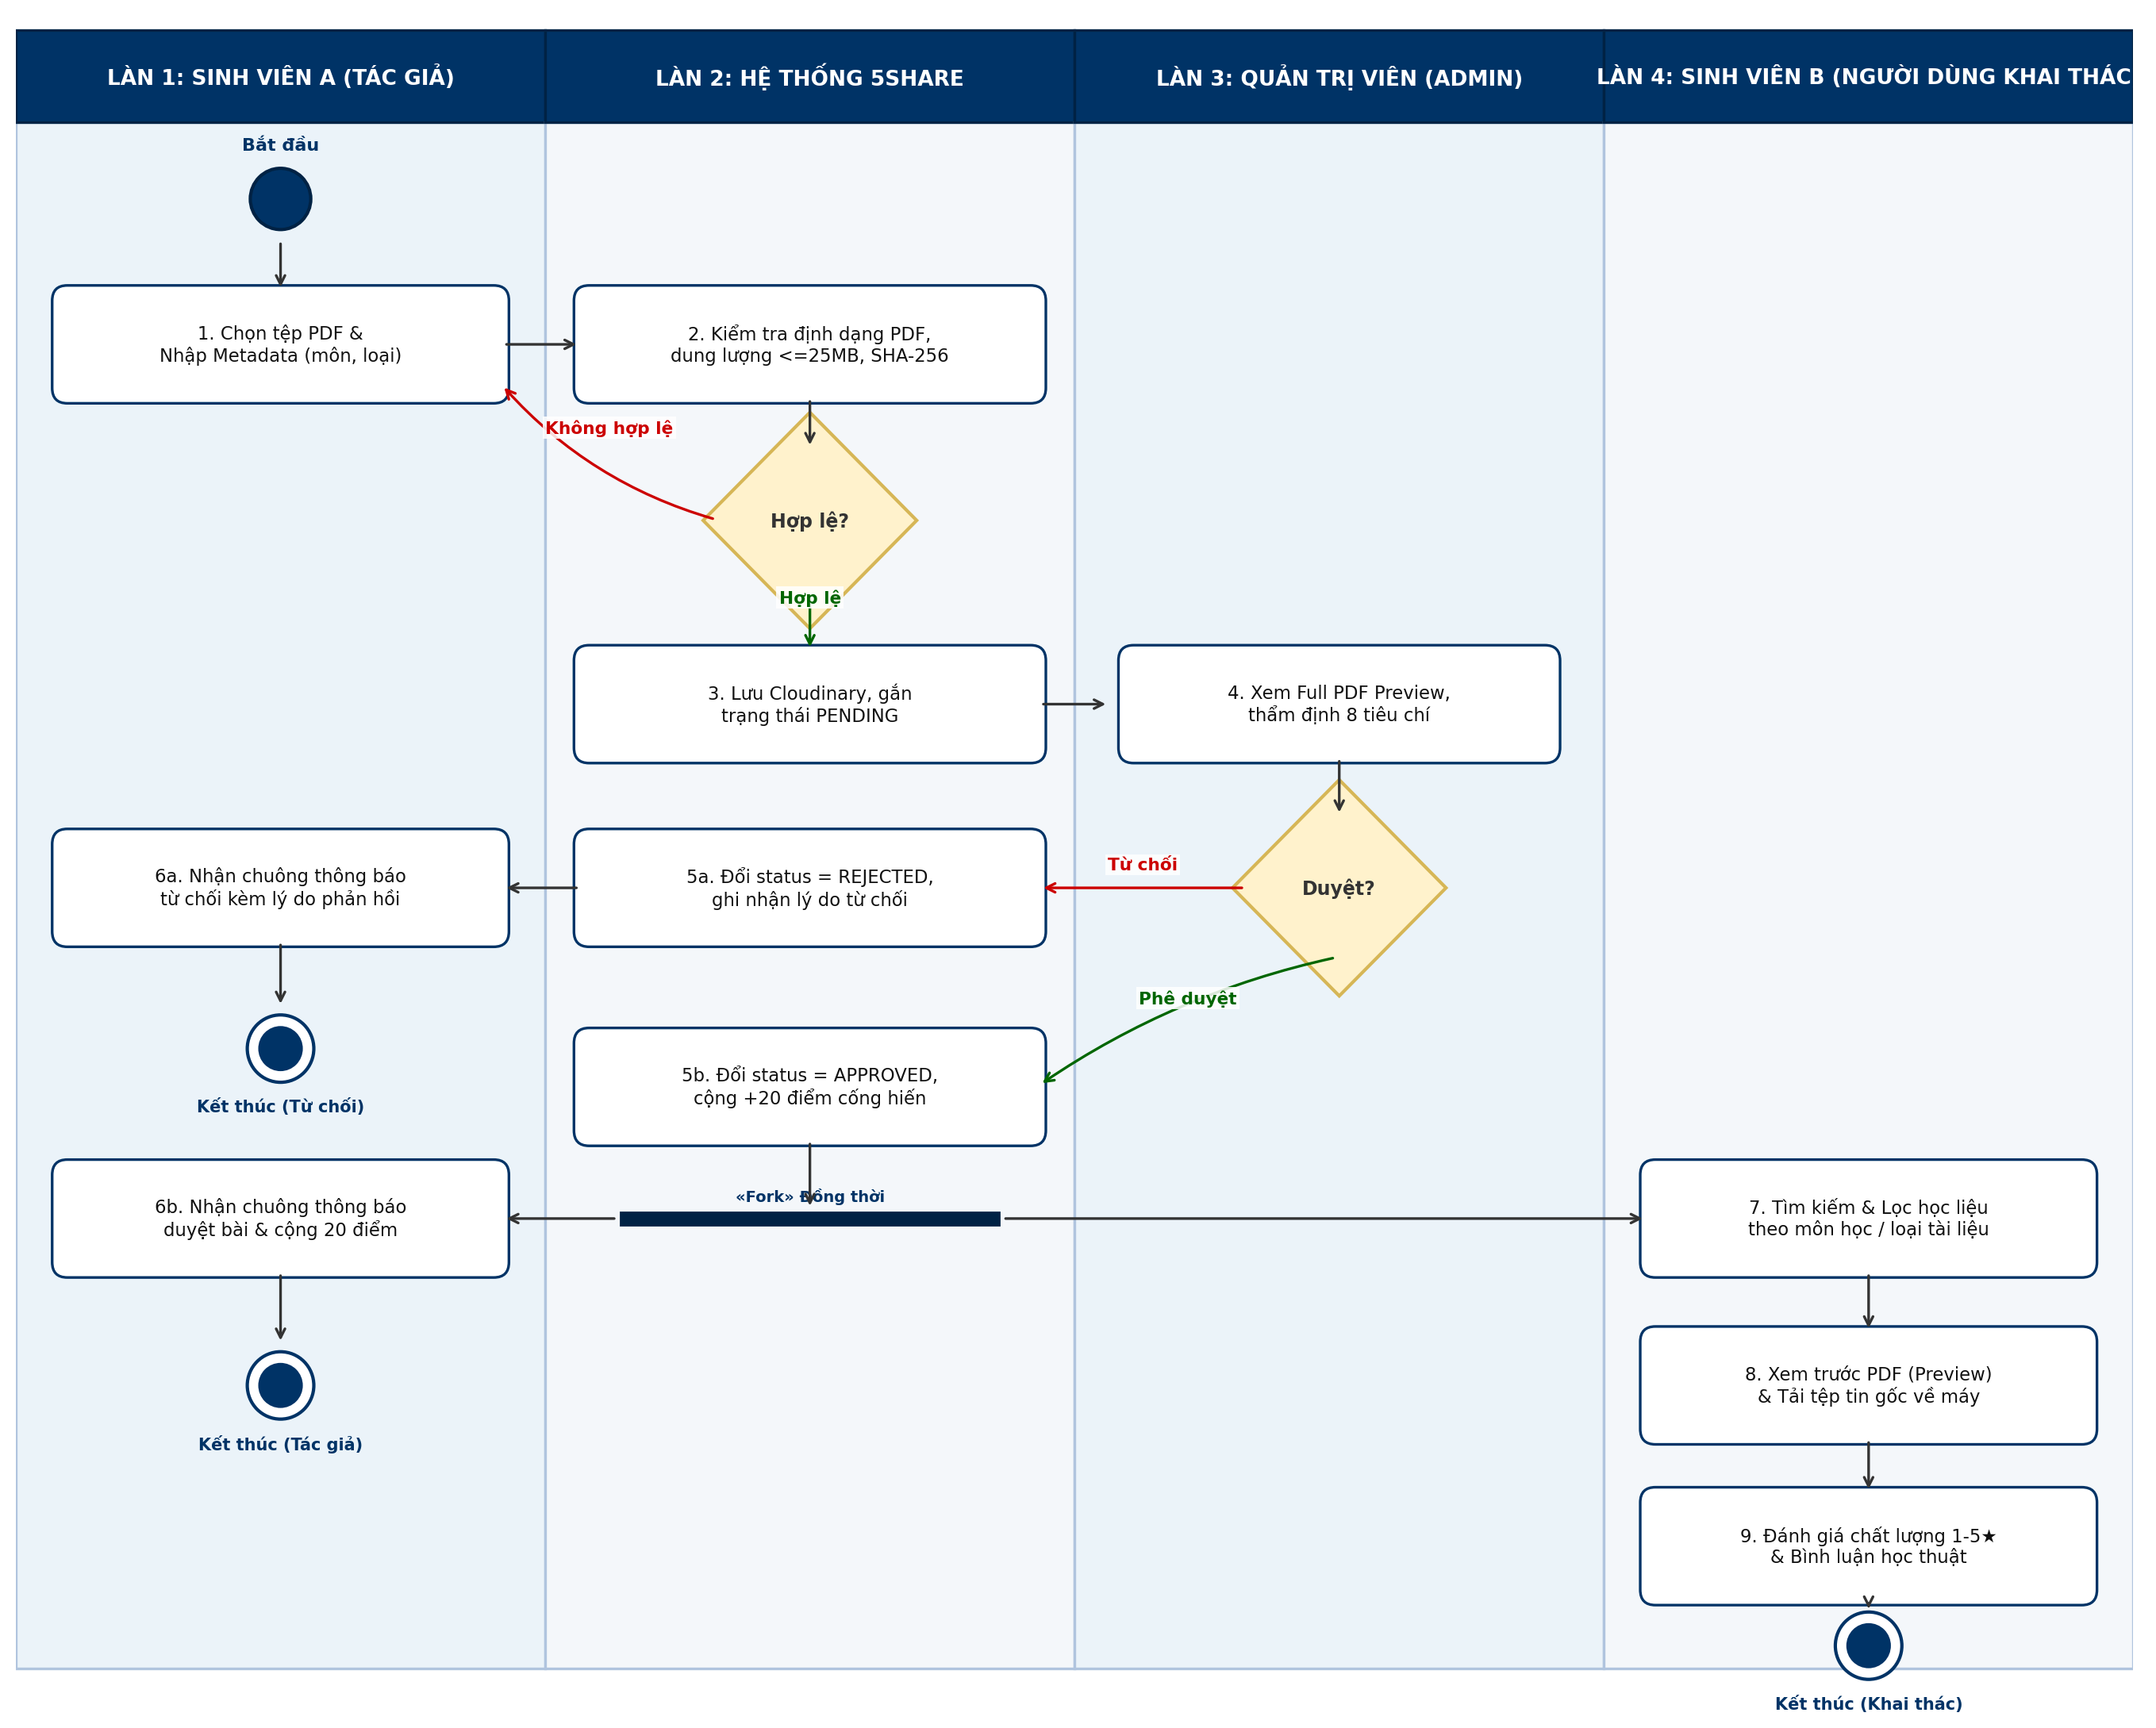
\includegraphics[width=0.98\textwidth]{chuong1/images/activity_swimlane_5share.png}%
}{%
    \IfFileExists{chuong1/images/hinh_1_3_activity.png}{%
        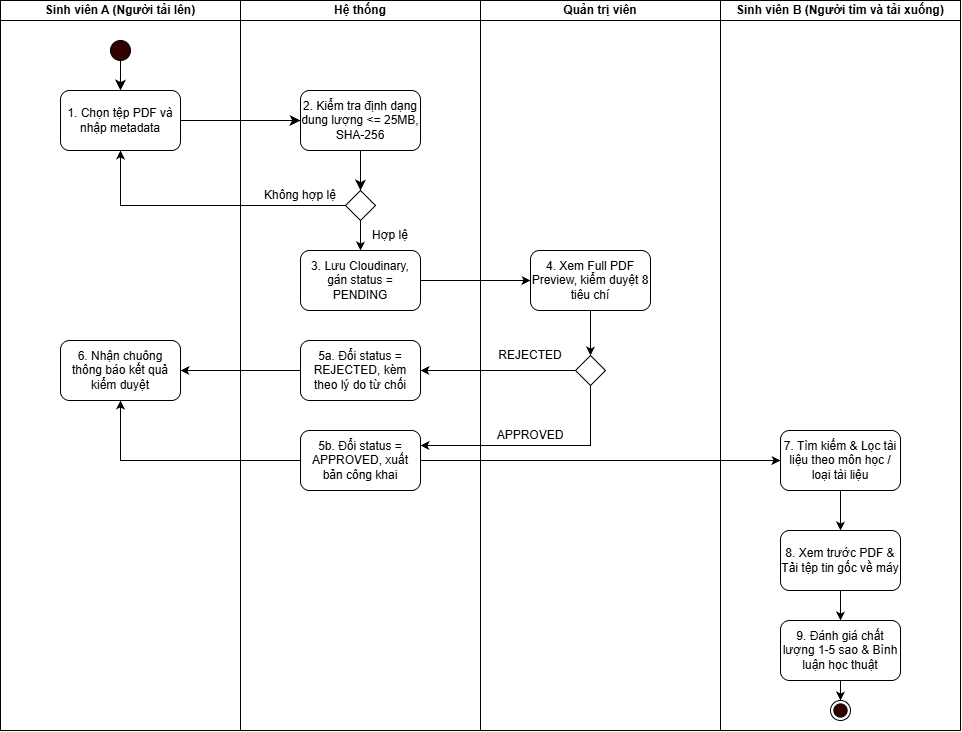
\includegraphics[width=0.98\textwidth]{chuong1/images/hinh_1_3_activity.png}%
    }{%
        \fbox{\parbox{0.95\textwidth}{\centering \vspace{3cm}\textbf{[Hình 1.3: Biểu đồ hoạt động mô tả nghiệp vụ của hệ thống 5Share]}\vspace{3cm}}}%
    }%
}
\caption{Biểu đồ hoạt động mô tả nghiệp vụ của hệ thống 5Share}
\label{fig:activity_swimlane}
\end{figure}

Biểu đồ trên thể hiện rõ quy trình khép kín gồm 3 giai đoạn phối hợp nghiệp vụ:
\begin{itemize}[leftmargin=*,noitemsep]
    \item \textbf{Giai đoạn 1 (Đăng tải \& Kiểm tra tự động):} Sinh viên chọn tệp tin PDF và nhập các metadata bắt buộc (tên tài liệu, môn học, phân loại, mô tả). Hệ thống tự động kiểm tra định dạng tệp tin, kiểm tra dung lượng, tính mã băm SHA-256 để đối chiếu chống trùng lặp, sau đó lưu trữ tệp lên máy chủ đám mây Cloudinary và thiết lập trạng thái ban đầu là PENDING.
    \item \textbf{Giai đoạn 2 (Kiểm duyệt):} Tài liệu chuyển vào hàng đợi kiểm duyệt của quản trị viên. Quản trị viên mở tài liệu, xem toàn văn bằng Full PDF Preview và kiểm duyệt theo 8 tiêu chí. Nếu đạt yêu cầu, quản trị viên phê duyệt chuyển trạng thái sang APPROVED để công khai; nếu không đạt, chuyển sang REJECTED kèm lý do cụ thể. Dù là chấp nhận xuất bản hay từ chối, hệ thống vẫn kích hoạt thông báo phản hồi về tài khoản của tác giả nhằm biết được trạng thái hiện tại của tài liệu mình đã tải lên.
    \item \textbf{Giai đoạn 3 (Khai thác \& Tương tác cộng đồng):} Người dùng khác truy cập kho học liệu, tra cứu và lọc tài liệu theo môn học. Khách vãng lai chỉ được đọc thử tối đa 3 trang đầu; sinh viên đã đăng nhập được đọc toàn văn, tải tệp tin gốc về máy, đồng thời tham gia đánh giá chất lượng và bình luận trao đổi nếu có ý kiến nào đó.
\end{itemize}

\subsubsection{1.4.2. Biểu đồ phân cấp chức năng}

\begin{figure}[H]
\centering
\IfFileExists{chuong1/images/bfd_diagram_5share.png}{%
    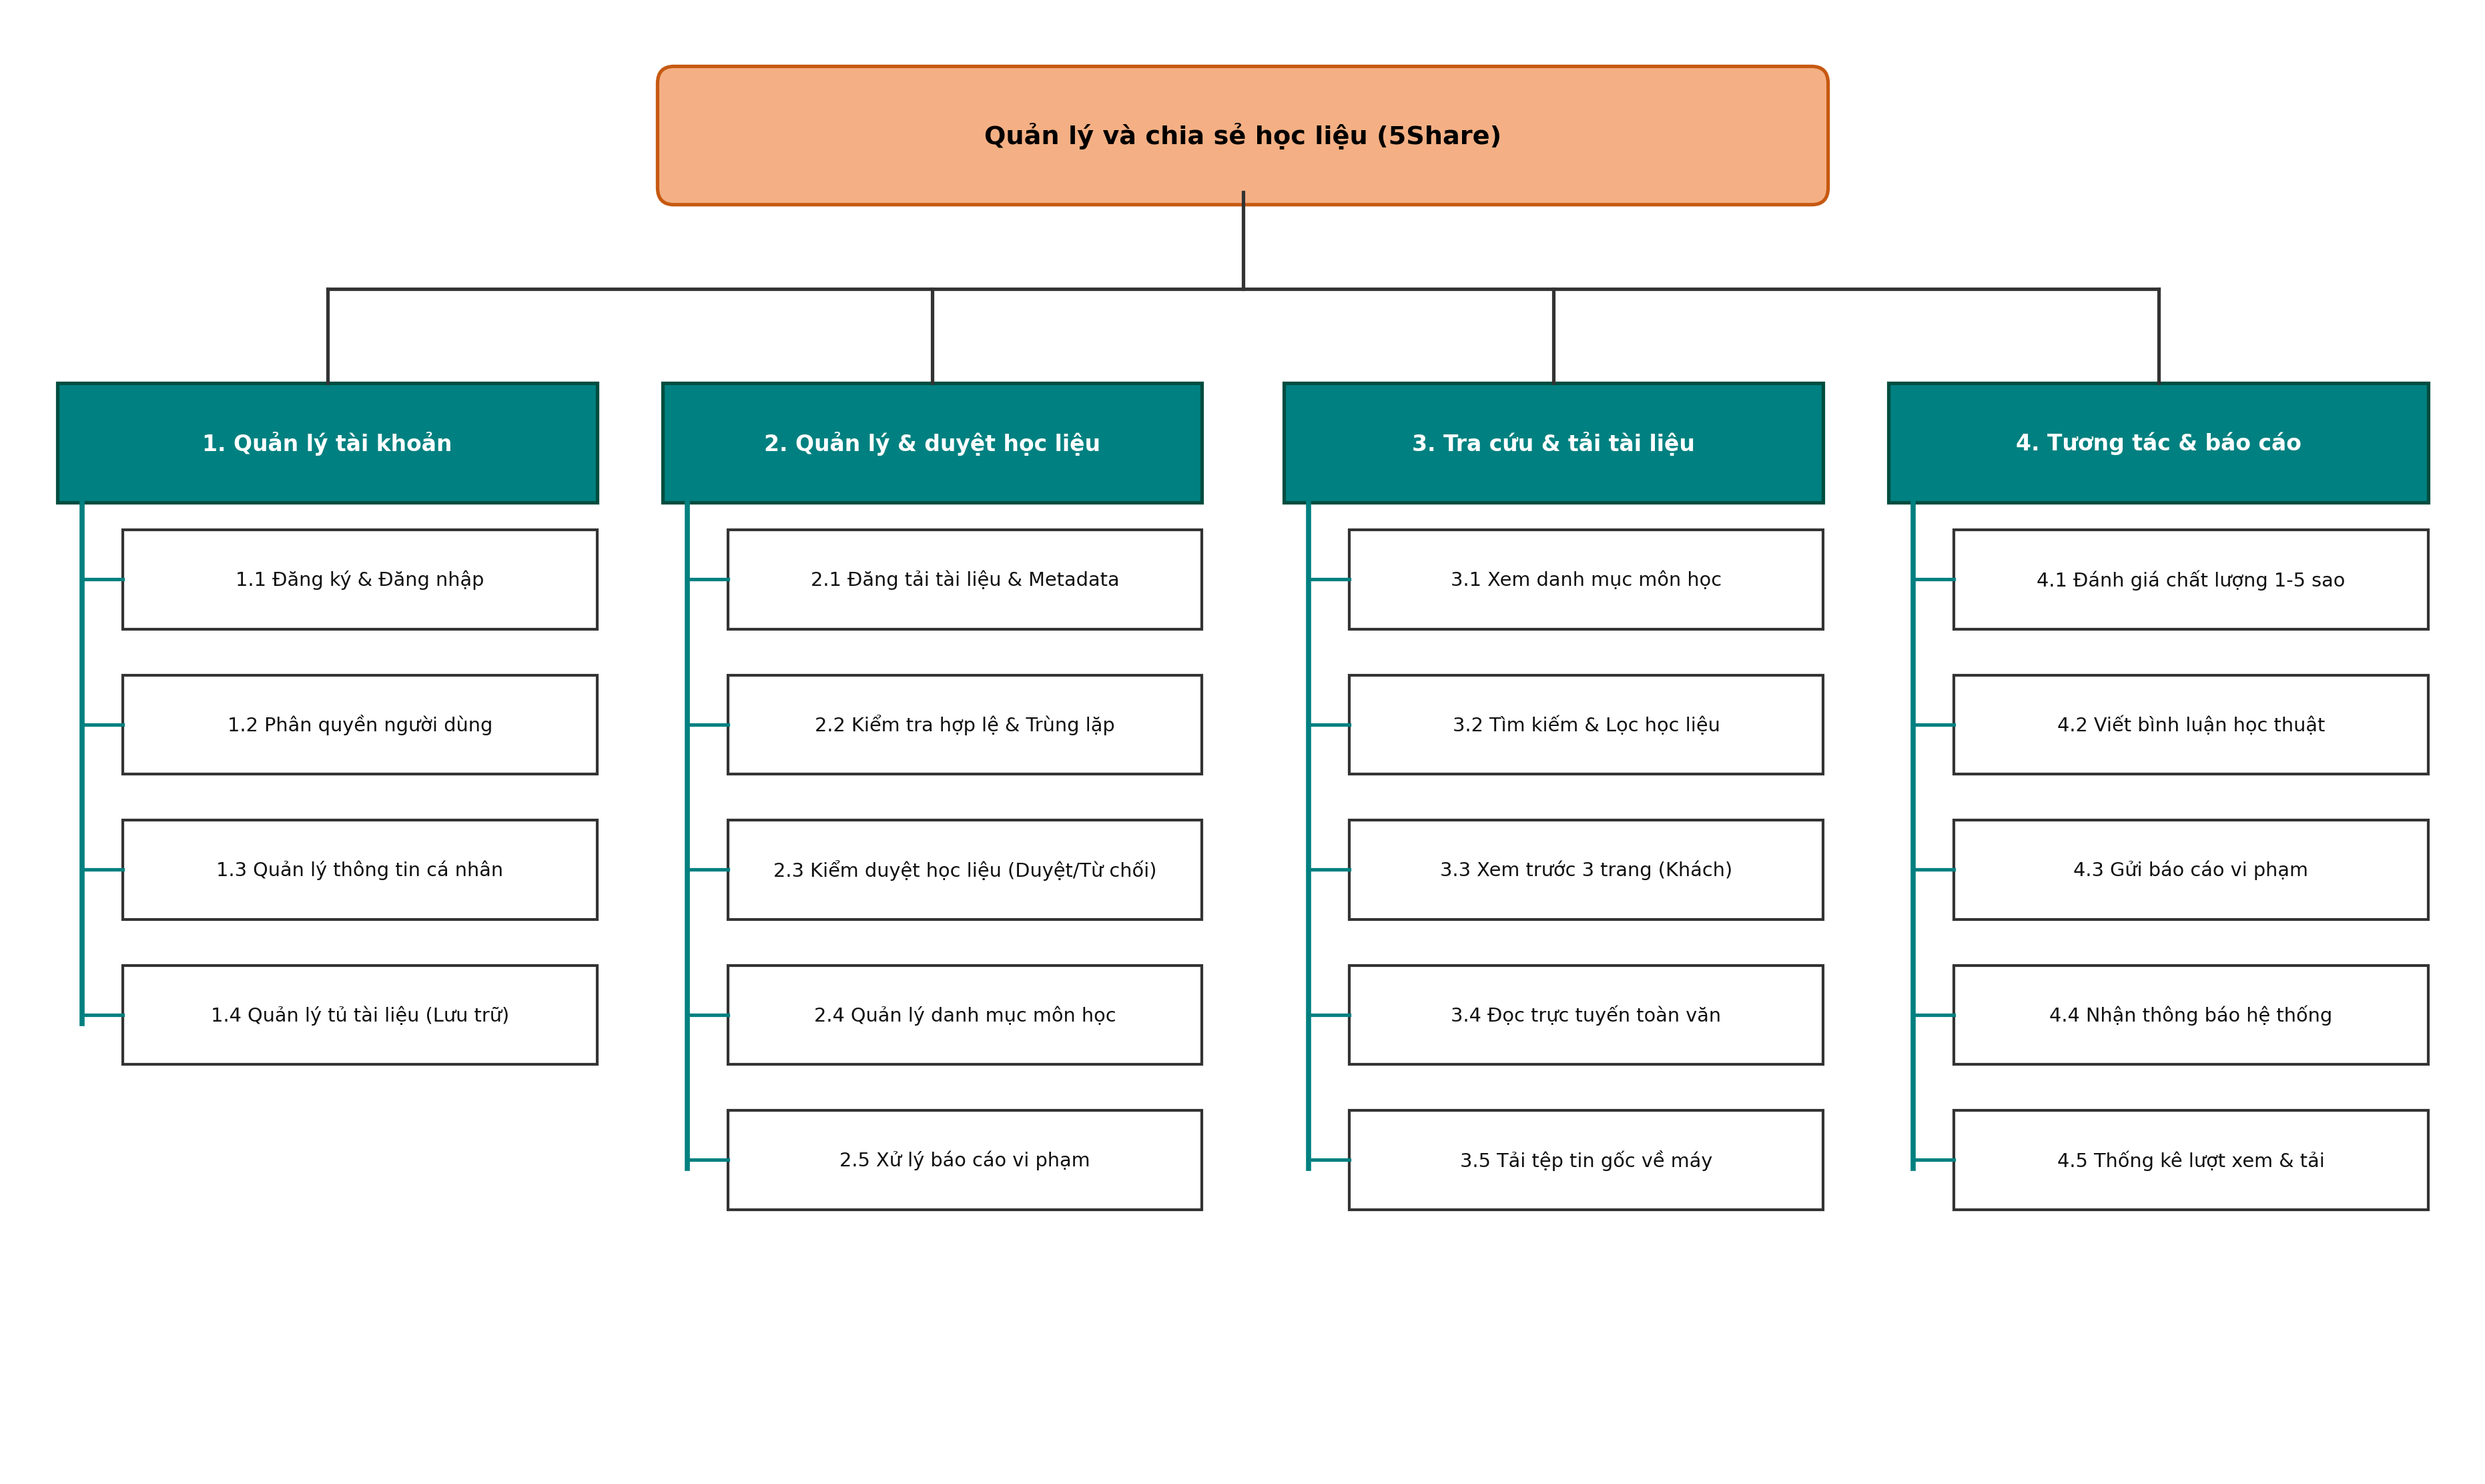
\includegraphics[width=0.98\textwidth]{chuong1/images/bfd_diagram_5share.png}%
}{%
    \IfFileExists{chuong1/images/hinh_1_4_bfd.png}{%
        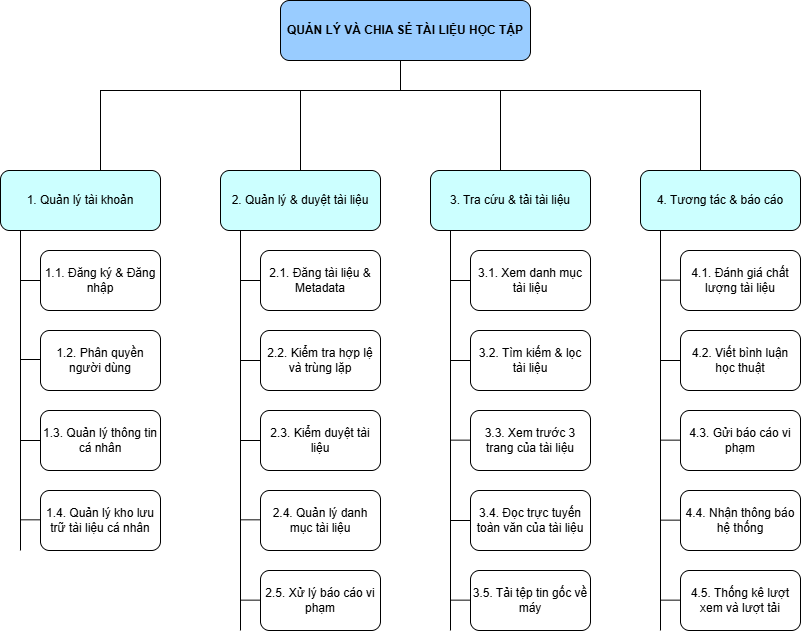
\includegraphics[width=0.98\textwidth]{chuong1/images/hinh_1_4_bfd.png}%
    }{%
        \fbox{\parbox{0.95\textwidth}{\centering \vspace{3cm}\textbf{[Hình 1.4: Biểu đồ phân cấp chức năng của hệ thống 5Share]}\vspace{3cm}}}%
    }%
}
\caption{Biểu đồ phân cấp chức năng của hệ thống 5Share}
\label{fig:bfd_tree}
\end{figure}

\subsubsection{1.4.3. Bảng mô tả chi tiết khối chức năng và đánh giá tính khả thi}
Tính khả thi của các khối chức năng được đánh giá toàn diện trên 4 phương diện: Nhân lực, Thời gian, Công nghệ và Môi trường vận hành như sau:

\begin{table}[H]
\centering
\small
\renewcommand{\arraystretch}{1.25}
\begin{tabularx}{\textwidth}{|p{3.2cm}|p{4.2cm}|X|}
\hline
\rowcolor[HTML]{EAEAEA}
\textbf{Khối chức năng} & \textbf{Mô tả} & \textbf{Đánh giá tính khả thi (nhân lực, thời gian, công nghệ, môi trường)} \\
\hline
\textbf{1. Quản lý tài khoản} & Đăng ký, đăng nhập JWT, quản lý phân quyền 3 vai trò (Guest, Student, Admin). Quản lý hồ sơ cá nhân và ``Tủ tài liệu cá nhân''. & 
- \textbf{Nhân lực:} 01 thành viên chính (Trâm) + Hỗ trợ backend (Khoa).\newline
- \textbf{Thời gian:} 2 tuần (Sprint 1).\newline
- \textbf{Công nghệ:} Node.js, Express, bcrypt băm mật khẩu, JWT token, PostgreSQL.\newline
- \textbf{Môi trường:} Tương thích trình duyệt web, lưu trữ token an toàn tại LocalStorage/HttpOnly Cookie. \\
\hline
\textbf{2. Quản lý \& duyệt tài liệu} & Upload PDF, validate Magic Bytes, băm SHA-256 check trùng lặp, hàng đợi chờ kiểm duyệt, duyệt/từ chối kèm lý do, quản lý loại tài liệu, xử lý báo cáo vi phạm. & 
- \textbf{Nhân lực:} 02 thành viên chính (Vĩ phụ trách Upload, Danh phụ trách Kiểm duyệt Admin).\newline
- \textbf{Thời gian:} 2.5 tuần (Sprint 1 \& Sprint 2).\newline
- \textbf{Công nghệ:} Multer, Cloudinary SDK, crypto (SHA-256), PostgreSQL Transaction.\newline
- \textbf{Môi trường:} Lưu trữ file đám mây an toàn, bảo vệ URL không để lộ tệp chưa duyệt. \\
\hline
\textbf{3. Tra cứu \& tải tài liệu} & Xem danh mục môn học theo CTĐT, Full-Text Search, phân trang, trình đọc PDF Preview giới hạn 3 trang cho Guest và toàn văn cho Student, luồng tải file gốc. & 
- \textbf{Nhân lực:} 02 thành viên chính (Khoa phụ trách Tìm kiếm, Đạt phụ trách Luồng tải \& Preview).\newline
- \textbf{Thời gian:} 2 tuần (Sprint 2).\newline
- \textbf{Công nghệ:} ReactJS, Tailwind CSS, PDF.js render canvas, PostgreSQL tsvector search.\newline
- \textbf{Môi trường:} Giao diện thích ứng tốt trên cả desktop và mobile. \\
\hline
\textbf{4. Tương tác \& báo cáo} & Đánh giá sao (1--5 sao) chống lặp, bình luận học thuật, báo cáo vi phạm, chuông thông báo hoạt động, Dashboard chứa biểu đồ thống kê tương tác và lượt tải. & 
- \textbf{Nhân lực:} 02 thành viên chính (Đạt phụ trách Đánh giá/Thống kê, Trâm phụ trách Thông báo).\newline
- \textbf{Thời gian:} 2 tuần (Sprint 3).\newline
- \textbf{Công nghệ:} Thư viện Recharts dựng biểu đồ thống kê, trigger PostgreSQL tạo thông báo.\newline
- \textbf{Môi trường:} Hiển thị trực quan, thời gian phản hồi API $<$ 500ms, giao diện hiện đại. \\
\hline
\end{tabularx}
\caption{Đánh giá tính khả thi của các khối chức năng theo 4 phương diện}
\label{tab:tinh_kha_thi}
\end{table}
